\documentclass[xcolor=dvipsnames,12pt]{beamer}
\usecolortheme[named=RoyalPurple]{structure}
\useoutertheme{infolines}
\usetheme{CambridgeUS}
%\usetheme[height=14mm]{Rochester}
%\hypersetup{colorlinks=true,linkcolor=yellow}
\setbeamertemplate{items}[ball]
\setbeamertemplate{blocks}[rounded][shadow=true]
\setbeamertemplate{navigation symbols}{}
\usepackage{color}
%\usefonttheme{structuresmallcapsserif}
%\usefonttheme{professionalfonts}
%\useoutertheme{default}
%\useoutertheme{infolines}


%\documentclass{beamer}
%\usecolortheme{structure}
\usepackage{graphicx}
%\usetheme{PaloAlto}
%\setbeamertemplate{items}[ball]
%\setbeamertemplate{blocks}[rounded][shadow=true]
%\useoutertheme{umbcfootline}
\newtheorem{assume}{\rlap{A}\hskip .1in}
%\newtheorem{result}{Result}[chapter]
\newcommand{\Var}  {\mbox{Var}}
\newcommand{\V} {\mbox{V}}
\newcommand{\E}  {\mbox{E}}
\newcommand{\PR}  {\mbox{P}}
\newcommand{\diag} {\operatorname*{diag}}
\newcommand{\tr} {\mbox{tr}}
\newcommand{\bmw}[1]{{\mbox{$#1$}}}
\newcommand{\MSE}{\mbox{MSE}}
\newcommand{\MSPE}{\mbox{MSPE}}


\def\bmh{{\hat \mathbf m}}
\def\bm{{\mathbf m}}
\def\bn{{\mathbf n}}
\def\mh{{\hat m}}
\def\bOmega{{\mathbf \Omega}}
\def\be{{\mathbf e}}
\def\bs{{\mathbf s}}
\def\by{{\mathbf y}}
\def\b1{{\mathbf 1}}
\def\bx{{\mathbf x}}
\def\bw{{\mathbf w}}
\def\bzero{{\mathbf 0}}

\def\bP{{\mathbf P}}
\def\bI{{\mathbf I}}
\def\bM{{\mathbf M}}
\def\bH{{\mathbf H}}
\def\bN{{\mathbf N}}
\def\bW{{\mathbf W}}
\def\bX{{\mathbf X}}
\def\bZ{{\mathbf Z}}
\def\bT{{\mathbf T}}
\def\bV{{\mathbf V}}
\def\bC{{\mathbf C}}
\def\bG{{\mathbf G}}
\def\bY{{\mathbf Y}}
\def\bD{{\mathbf D}}
\def\bS{{\mathbf S}}
\def\bR{{\mathbf R}}

\def\bbeta{\mbox{\boldmath $\beta$}}
\def\bepsilon{\mbox{\boldmath $\varepsilon$}}

% items enclosed in square brackets are optional; explanation below
\title[]{Part 2}
%\subtitle[ttt]{}
\author[Stat 801]{Random Variables, Probability Distributions\\
Binomial Distribution\\
Normal Distribution, Standard Normal Distribution\\
The Central Limit Theorem\\
Poisson Distribution}
\date{}

\begin{document}

\begin{frame}[plain]
  \titlepage
\end{frame}


\begin{frame}
\frametitle{Population versus Sample}
\textcolor{blue}{Population} -- The set of all objects under consideration.
Objects in a population are called  \textcolor{magenta}{\textit{elements}}.\\
 \textcolor{blue}{Examples}
\begin{itemize}
\item  Boxes of a particular brand of corn flakes. 
\item  Newly made light bulbs in a warehouse at a given time.
\end{itemize}
\end{frame}



\begin{frame}
\frametitle{Another Definition of Population}
\begin{itemize}
\item All possible outcomes of an  \textcolor{magenta}{\textit{experiment}} can also be values
in a population.
\item Flipping a coin twice.  Possible outcomes are:\\ HH, HT, TH, TT.
Could  make the outcomes numeric using 3, 2, 1, 0 to be the elements
corresponding to the above \textcolor{magenta}{events}. 
\item If the experiment is repeated many times, the resulting values
constitute a population: $2,\ 0,\ 3,\ 1,\ 0,\ 2,\ \dots$
\end{itemize}
\end{frame}


\begin{frame}
\frametitle{Random Sampling}
\begin{itemize}
\item \textcolor{magenta}{Sample} -- A subset of the elements from a population.
\item \textcolor{magenta}{Simple Random Sample} of size $n$ from a \textcolor{magenta}{finite 
population} is a  subset selected in such a way that every subset of 
$n$ elements is equally likely to be the one selected. (Abbreviation: SRS)
\item A random sample from a small finite population can be obtained using the
\textcolor{magenta}{Random Numbers} - using code or random number table.
\begin{itemize}
\item sample(1:100,3) or sample(3)
\end{itemize}
\item Computer programs are used to draw samples from large populations.
\end{itemize}
\end{frame}


\begin{frame}
\frametitle{Probability, Random Variables, and\\ Probability Distributions}
\begin{itemize}
\item Assume a numeric finite population  of $N$ elements, and suppose $n_1$
of the elements are the number $k$.
\item Suppose a SRS of size 1 is taken from this population.
\item The \textcolor{magenta}{probability} that the number $k$ is selected is $n_1/N$.  
\item That is, we define this probability to be the relative frequency of
occurrence of $k$ in the population.
\end{itemize}
\end{frame}


\begin{frame}
\frametitle{Probability: Example}
\begin{itemize}
\item {\textcolor{blue}{Example:}} \ \ $N = 10$
\item {\textcolor{blue}{Population}}:  1, 1, 1, 3, 7, 7, 9, 9, 9, 9
\item Denote by $P(k)$, \textcolor{magenta}{the probabilty of the number k being selected}
\item  $P(1) = 3/10$,\ \  $P(3) = 1/10$,\ \  $P(7) = 2/10$,\\ 
$P(9) = 4/10$,\ \  $P(2) = 0/10$,\ \  $P(1~\mbox{or}~3) = 4/10$, \\
$P(\mbox{not}~7) = 1-2/10$.
\end{itemize}
\end{frame}


\begin{frame}
\frametitle{Random Variables}
A {\textcolor{blue}{random variable}} is a function defined on a numeric
population.  We will often say that this function value is 
\textcolor{magenta}{the value assumed by the random variable}.
\begin{itemize}
\item {\textcolor{blue}{Example}}: $N = 10$ 
\item {\textcolor{blue}{Population}}:  1, 1, 1, 3, 7, 7, 9, 9, 9, 9
\item Let $X$ be a random variable defined on this population.  
\item $X$ can assume any of the values 1, 3, 7, or 9.
\end{itemize}
\end{frame}
 

\begin{frame}
\frametitle{Random Variables (continued)}
\begin{itemize}
\item A {\textcolor{blue}{Random variables}} are different from
ordinary variables because they assume values from the population
with associated probabilities. 
\item For e.g., we will say \\[.01in] 
\ \ \ $P(X=1)=3/10$,\ \ \ $P(X=7)=2/10$, \\
\ \ \ $P(X=2)=0/10$,\ \ \ $P(X=-6)=0/10$, \\
\ \ \ $P(1 \leq X \leq 3)=4/10$,\ \ \ $P(1 \leq X \leq 9)=1$. etc.
\item A \textcolor{magenta}{probability distribution} specifies the
probabilities  associated with all possible values the
random variable $X$ can assume.\\
\end{itemize}
\end{frame}



\begin{frame}
\frametitle{The M \& M Example}
\textcolor{blue}{Example}:\\
If X represents the number of RED $M\&Ms$ in a vending machine size
package, then perhaps \textcolor{magenta}{the probability distribution of $X$} is 
something like the following:\\

\begin{tabular}{|c|ccccccc|}
\hline
$x$ & 5 & 6 & 7 & 8& 9& 10 & 11 \\ \hline
$P(X=x)$ &
$\frac{2}{28} $ & $\frac{2}{28}$ & $\frac{5}{28}$ & $\frac{7}{28}$ &
$\frac{5}{28} $ & $\frac{4}{28}$ & $\frac{3}{28}$ \\ \hline
\end{tabular}
\end{frame}


\begin{frame}
\frametitle{The M $\&$ M Example (continued)}
  We read this table by finding a value of X, say 8, then 
reading the probability below it: 
\begin{itemize}
\item \textcolor{magenta}{The probability of observing 8 M$\&$Ms in a package is
$\frac{7}{28}$, meaning, if we open many many packages of M$\&$Ms,
about 7 out of 28 will have exactly 8 M\&Ms within.}
\end{itemize}
This is an example of a \textcolor{magenta}{discrete random variable}.
\end{frame}


\begin{frame}
\frametitle{Discrete Random Variables}
\begin{itemize}
\item When the elements of a population consists of a countable
discrete set of values the random variable defined on that
population is called \textcolor{magenta}{discrete random variable}.
\item For discrete random variables the probability
distribution can be displayed using a histogram  or a table of
values and associated probabilities as shown above.
\end{itemize}
\end{frame}


\begin{frame}
\frametitle{The M \& M Probability Distribution}
%**************************************************************
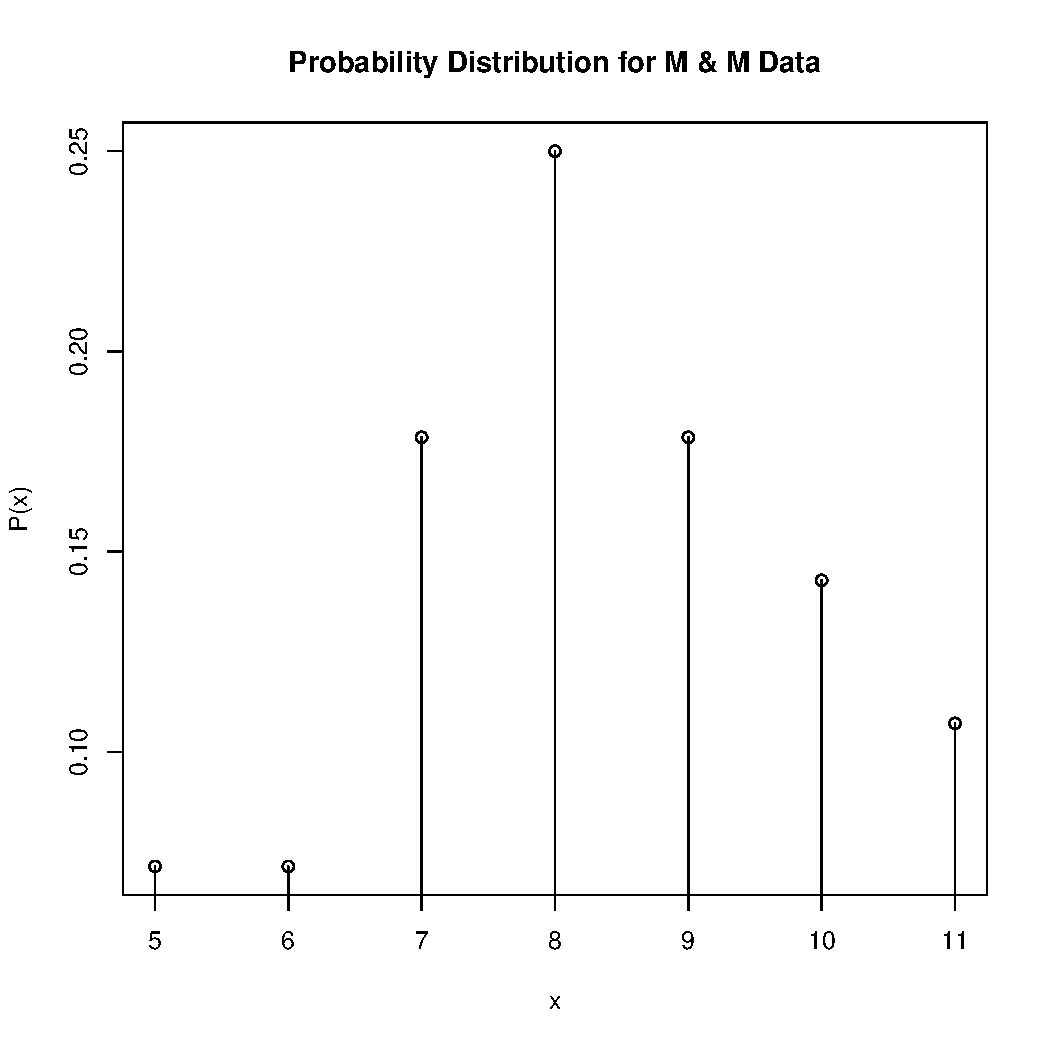
\includegraphics[scale=0.43]{prob_dist_MandM.pdf}
%**************************************************************
\end{frame}


\begin{frame}
\frametitle{Continuous Random Variables}
\begin{itemize}
\item When the population consists of an uncountable number of values
in a line interval use integration to calculate
proportions of the population that exist in any given
\textcolor{magenta}{subinterval} of a continuum.
\item  For a random variable defined on
such a population we will deal with the probability that the random
variable assumes a value in a given interval, not that it assumes a
specific numeric value.
\end{itemize}
\end{frame}

\begin{frame}
\frametitle{Continuous Random Variables (contd.)}
\begin{itemize}
\item When the population consists of a set of values in a continuous range
the random variable defined on that population is called 
\textcolor{magenta}{continuous random variable}.
\item The probability distribution of a  continuous
random variable is a smooth curve. 
\item The \textcolor{magenta}{area under the curve} between
specified values of the random variable correspond to a
probability.
\item The probability that a continuous random variable assumes
a specific numeric value is zero.
\end{itemize}
\end{frame}


\begin{frame}
\frametitle{Continuous Random Variables (contd.)}
\begin{itemize}
\item \textcolor{blue}{Example:} A Continuous Random Variable $X$ defined on 
\item a \textcolor{magenta}{Population}: all numbers in the interval (0,2) occurring with various
frequencies (that we won't specify here).
\item By Definition\\
$P(1/2 \leq X \leq 1/2) \equiv P(X = 1/2) = 0$ \\
$P(0 \leq X \leq 2) = 1,\ \ \ P(X < 0) = P(X \leq 0) = 0$ 
\item  We could possibly calculate the following probability\\ $P(1 \leq X \leq 2) = ?$
\end{itemize}
\end{frame}


\end{document}
\begin{frame}
\frametitle{Binomial Random Variable}
\begin{itemize}
\item For some interesting populations that occur naturally, theoretical
probability distributions and associated random variables, have
been defined. 
\item One such population features elements that are only
one of two kinds (Yes or No; \ Good or Defective; \ Below or
Above;, etc.).
\item Let us use \textcolor{green}{Success(S)} and \textcolor{red}{Failure(F)} to designate population
elements, in general
\item Consider a typical population of this kind consisting of 
$m$ \textcolor{green}{S}'s and $N-m$ \textcolor{red}{F}'s, where $N$ is the total number of elements in
the population.
\end{itemize}
\end{frame} 


\begin{frame}
\frametitle{Binomial Experiment}
\begin{itemize}
\item A \textcolor{magenta}{binomial experiment} consists of taking $n$ successive SRS,
each of size 1, replacing elements between draws, and counting
the number of \textcolor{green}{S}'s obtained.
\item The binomial experiment is conducted by sampling from the population
of \textcolor{green}{S}'s and \textcolor{red}{F}'s. 
\item The proportion of \textcolor{green}{S}'s in the population is $\pi = m/N$ 
so the proportion of \textcolor{red}{F}'s is $1 - \pi \equiv (N-m)/N$.
\item Let $X_i$ be the random variable that assumes the value of the
outcome of the $i$-th draw  for each $i=1,2,\ldots,n$. 
\end{itemize}
\end{frame}


\begin{frame}
\frametitle{Binomial Distribution}
\begin{itemize}
\addtolength{\itemsep}{-0.6\baselineskip}
\item Let the random variable  $X_i$ assume the value 1 if the outcome of the
 $i$-th draw  is \textcolor{green}{S} or the  value 0 if the outcome  is \textcolor{red}{F}. \\[.1in]
\item Thus we imagine $n$ random variables,  $X_1, X_2, X_3, \ldots, X_n$ each assuming a 
value \textcolor{green}{S} with probability $\pi$, or \textcolor{red}{F} with probability $1 - \pi$.\\[.1in]
\item That is, the probability distribution of \textit{each} of the $n$ random variables
 $X_1, X_2, X_3, \ldots, X_n$ is given by:\\[.1in]
\begin{tabular}{|c|cc|}
\hline
$x$ & 0& 1 \\ \hline
$P(X=x)$ & $1-\pi$ & $\pi$ \\ \hline
\end{tabular}
\end{itemize}
\end{frame}




\begin{frame}
\frametitle{Binomial Distribution (contd.)}
\begin{itemize}
\addtolength{\itemsep}{-0.6\baselineskip}
\item Now define a new random variable $Y$ so that
$$
  Y = X_1 + X_2 + X_3 + \cdots + X_n \, 
$$
\item $Y$ represents the number of \textcolor{green}{Success(S)}'s in the set of values assumed by 
$X_1,\ X_2, \ldots,X_n$.  \\[.1in]
\item This is because each $X_i=1$ when an \textcolor{green}{S} is drawn,
and  $X_i=0$  otherwise, we can see that $Y$ represents the total number of 
\textcolor{green}{S}'s in the experiment. \\[.1in]
\item $Y$ is said to be a  \textcolor{magenta}{binomial random variable}.
\end{itemize}
\end{frame}



\begin{frame}
\frametitle{Binomial Distribution (contd.)}
\begin{itemize}
\addtolength{\itemsep}{-0.6\baselineskip}
\item That is, a \textcolor{magenta}{binomial random variable}  assumes the value of the
total number of successful outcomes in a binomial experiment.\\[.1in]
\item The random variable $Y$  can assume any one of the values 
0, 1, 2, $\ldots, n$ with a probability that
will depend on $n$, the number of samples  taken and $\pi$.\\[.1in]
\item $Y$ is said to be the Binomial ($n,\pi$) random variable.\\[.1in]
\item A population on which $Y$ is defined consists of the unique elements
$0,1,2,\ldots,n$. \\[.1in]
\item What is the proportion of each element in the population?
i.e., What is the probability that $Y$ assumes each value?
\end{itemize}
\end{frame}



\begin{frame}
\frametitle{Binomial Distribution (contd.)}
Theoretically, for any finite $n$, the probability that a\\
\textcolor{magenta}{binomial random variable} $Y$ takes on values 0, 1, 2, $\dots, n$\\ 
is given by\\
\begin{eqnarray*}
P(Y=y) & = & \frac{n!}{y!(n-y)!}\pi^y\,(1 - \pi)^{n-y}, \\
\mbox{where} & & \\
        y & = & 0, 1, 2, \ldots, n \mbox {(number of successes in n trials)}\\
\pi & = &  \mbox{ probability of success in a single trial}\\
1-\pi & = &  \mbox{ probability of failure in a single trial}\\
n! & = & n(n-1)(n-2) \ldots (3)(2)(1)
\end{eqnarray*}
\end{frame}


\begin{frame}
\frametitle{Binomial Distribution (contd.)}
\begin{itemize}
%\addtolength{\itemsep}{-0.6\baselineskip}
\item In applications, we won't know $\pi$ and our objective will
usually be to sample the population in order to \textcolor{magenta}{estimate}
$\pi$, and get an idea about the \textcolor{magenta}{error} in that estimate.
\item What is the \textcolor{magenta}{mean} $\mu$ and
\textcolor{magenta}{variance} $\sigma^2$ (or the standard deviation $\sigma$
of a binomial random variable?
\item In general, for a \textcolor{magenta}{discrete random variable}, these are defined is as follows.\\[.1in]
\end{itemize}
\end{frame}

\begin{frame}
\frametitle{Computing the Mean and Variance of a Discrete Random Variable}
\begin{itemize}
\addtolength{\itemsep}{-0.7\baselineskip}
\item The \textcolor{magenta}{mean} of a discrete random variable $X$ is:
$$
  E(X) = \mu = \sum_x\,x \cdot P(X=x)
$$
\item The \textcolor{magenta}{variance} of a discrete random variable $X$ is:
$$
  V(X) = \sigma^2= \sum_x\,(x - E(X))^2. \ P(X=x) 
$$
\item The \textcolor{magenta}{standard deviation} of a random variable  $X$ is
$$\sqrt{V(X)}=\sigma$$
\end{itemize}
\end{frame}


\begin{frame}
\frametitle{Computing the Mean and Variance of a Binomial Random Variable}
\begin{itemize}
%\addtolength{\itemsep}{-0.6\baselineskip}
\item  Using the above formula, the \textcolor{magenta}{mean} of 
a Binomial random variable \ $Y$, is shown to be $E(Y)=\mu = n \, \pi$ 
\item The \textcolor{magenta}{variance} is shown to be $V(Y) =\sigma^2= n\,\pi(1 - \pi)$. 
\item Thus the 
\textcolor{magenta}{standard deviation} of a Binomial random variable is 
$\sigma= \sqrt{n\,\pi(1 - \pi)}$
\end{itemize}
\end{frame}


\begin{frame}
\frametitle{Binomial Distribution: Example}
 Consider a Binomial population with
$n=3,\ \pi = \frac13$,\\[.01in] 
i.e., $Y\ \sim\ \mbox{Bin}(3,\,\frac13)$, The corresponding Binomial distribution is\\
\begin{eqnarray*}
  P(0) &=& \frac{3!}{0!3!} \left(\frac13 \right)^0 \left( \frac23
           \right)^3 = 8/27\\[.1in]
  P(1) &=&  \frac{3!}{1!2!} \left(\frac13 \right)^1 \left( \frac23
           \right)^2 = 3 \cdot \left( \frac13
           \right)\, \left(\frac49 \right) = 12/27 \\[.1in]    
  P(2) &=&  \frac{3!}{2!1!} \left(\frac13 \right)^2 \left( \frac23
           \right) = 3 \cdot \left( \frac19
           \right)\, \left(\frac23 \right) = 6/27 \\[.2in]
  P(3) &=& 1 - P(0) - P(1) - P(2) = 1/27
\end{eqnarray*}
\end{frame}


\begin{frame}
\frametitle{Binomial Distribution: Example (contd.)}
The mean and variance of a Bin($3,\frac{1}{3}$) population is:
\begin{itemize}
\item Mean  $ = n \, \pi =  3 \times\frac{1}{3} = 1 $
\item Variance $  =  n\,\pi(1 - \pi) =  3 \times\frac{1}{3}\times\frac{2}{3} =
\frac{2}{3} $ 
\item Standard Deviation $ = \sqrt{.66667} = .8165$
\end{itemize}
\end{frame}



\begin{frame}
\frametitle{Using the Binomial Distribution}
\begin{itemize}
\item So how can this Binomial probability distribution benefit us?  
\item When sampling situation fits the requirements of a Binomial experiment, 
(at least approximately) we can view the results we obtain as the 
values assumed by a binomial random variable.  
\item This permits us to find probabilities of various
possible outcomes, and use these and other properties of a
binomial random variable to make inferences. 
\item To assume the \textcolor{magenta}{Binomial Model}, we need to determine whether
the values of the population elements are obtained as a result of a
\textcolor{magenta}{Binomial Experiment}. 
\end{itemize}
\end{frame}


\begin{frame}
\frametitle{The Binomial Model}
\begin{enumerate}
\item $n$ identical trials are made. 
\item Each trial results in either \textcolor{green}{Success($S$)} or
      \textcolor{red}{Failure($F$)}.  (only two possible outcomes).
\item The probability of success ($\pi$) remains the
      same from trial to trial.
\item The trials are independent.
\item Interest is in the number of successes obtained in the
      $n$ trials.  The number is viewed as being the value 
      assumed by a Binomial ($n,\ \pi$) random variable $Y$.
\end{enumerate}
\end{frame}


\begin{frame}
\frametitle{The Binomial Model}
\begin{itemize}
\item Requirement Number 3 in the definition of a binomial experiment
is usually the most difficult to satisfy in practical applications.
\item As trials are made, if selected elements are not replaced in the
sampled population, $\pi$ changes in value.
\item  If the population is
very large, the change is very small and can be ignored.
\end{itemize}
\end{frame}

\begin{frame}
\frametitle{Binomial Model: Are requirements satisfied? - Example 1}
An article in the March 5, 1998, issue of The New England Journal of Medicine discussed a large outbreak of tuberculosis. One person, called the index patient, was diagnosed with tuberculosis in 1995. The 232 co-workers of the index patient were given a tuberculin screening test. The number of co-workers recording a positive reading on the test was the random variable of interest. Did this study satisfy the properties of a binomial experiment?
\end{frame}

\begin{frame}
\frametitle{Binomial Model: Are requirements satisfied? - Example 1}
\begin{enumerate}
\item $n$ identical trials? Yes, $n=232$ workers
\item  Population of only $S$'s and $F$'s?   Yes.
\item Is probability of success same in each trial? Yes if we assume the co-workers had the same risk factors as the index patient.
\item Independent trials? Yes, the outcome of one screening was unaffected by the outcome of the other tests.
\item Was the random variable of interest to the experimenter the number of successes $y$ in the 232 screening tests? Yes, the number of co-workers who received a positive result.
\end{enumerate}
\end{frame}


\begin{frame}
\frametitle{Binomial Model: Are requirements satisfied? - Example 2}
An economist interviews 75 students in a class of 100 to estimate the proportion of student who expect to obtain a C or better in the course. Is this a binomial experiment?
\end{frame}

\begin{frame}
\frametitle{Binomial Model: Are requirements satisfied? - Example 2}
\begin{itemize}
\item  Population of only $S$'s and $F$'s?   Yes.
\item Is probability of success same in each trial? This may change
from trial to trial as we may not assume sampling with replacement.
\end{itemize}
\end{frame}



\begin{frame}
\frametitle{Binomial Example}
 A labor union's examining board for the selection of apprentices
has a record of admitting 70\% of all applicants who satisfy
a basic set of requirements.  Five members of a minority group,
all satisfying the requirements, recently came before the board,
and four of the five were rejected.  Find the probability that
1 or fewer would be accepted if the admission rate is really
0.70.
\end{frame}

\begin{frame}
\frametitle{Binomial Example - cont.}
\begin{itemize}
\item Board decisions are viewed as random draws from a
population consisting of $70\%$ Accepts (S) and $30\%$ Rejects (F).
\item We can assume a large population so that the probability of being
accepted remains constant across draws. 
\item Then the Binomial (5,0.7)
distribution is applicable to the number of Accepts in
$n=5$ trials with $\pi=0.7$.
\end{itemize}
\end{frame}


\begin{frame}
\frametitle{Binomial Example - cont.}
\begin{itemize}
\item Let $X$ be the random variable representing the number of Accepts,
and assume that $X$ has a Binomial (5, 0.7) distribution. Then
P(X=0) + P(X=1) =\\
${5}\choose{0}$ $(0.7)^0(0.3)^5+$ ${5}\choose{1}$ $(0.7)(0.3)^4=0.03078$
\item The probability that the board will accept fewer than 2 applicants
from a group of 5 is 0.03078 (which is a small probability)
\textcolor{magenta}{if indeed the true acceptance rate is 0.7.}
\end{itemize}
\end{frame}





\begin{frame}
\frametitle{Binomial Example - cont.}
\begin{itemize}
\item But in fact the board DID accept fewer than 2 of the group
of 5 so ...........
\item \textcolor{magenta}{Conclusion:}  Either the board was operating to admit
at its historical 70\% rate and we have simply witnessed an
extremely rare event, \textcolor{magenta}{or} 
\item  the board has changed policy and is currently admitting at
a rate less than 70\%. 
\item One would tend to favor the latter conclusion.
\end{itemize}
\end{frame}


%***************************************************************


\begin{frame}
\frametitle{Normal Random Variable}
\begin{itemize}
\item The \textcolor{magenta}{Normal probability distribution} is an
example of a  continuous distribution. 
\item The associated random
variable is defined in the interval (-$\infty,\infty)$.
\item To model the probability distribution of many  populations
we often use the Normal distribution. 
\item Most population \textcolor{magenta}{distributions} are bell-shaped and can be
modeled by the Normal distribution. 
\item We say that
the  associated \textcolor{magenta}{random variable} $X$, say, \\
\center{ $X \, \sim \, N(\mu,\, \sigma^2)$.}
\item Here $\mu$ and $\sigma$, are \textcolor{magenta}{parameters}
of the population. 
\end{itemize}
\end{frame}

\begin{frame}
\frametitle{Properties of the Normal Distribution}
\begin{itemize}
\item Probability function (or curve) of a
Normal random variable $X$ is
\begin{equation*}
  f(x) = \frac{1}{\sigma \sqrt{2\pi}} \, e^{- \frac{1}{2} \left(\frac{x-\mu}{\sigma}\right)^2}
\end{equation*}
where

\item $E(X)= \mu$ = mean : measures the \textcolor{magenta}{center of the distribution}.

\item $V(X)= \sigma^2$ = variance : \textcolor{magenta}{measures the spread}.

\item $\sqrt{V(X)}= \sigma$ = standard deviation : \textcolor{magenta}{measures the spread in
same units as the mean}.
\item $\pi$ = 3.1415\ldots \hspace*{3mm} $e$ = 2.71828\ldots
\end{itemize}
\end{frame}


\begin{frame}
\frametitle{Properties of the Normal Distribution (contd.)}
\begin{itemize}
\item The Normal distribution is symmetric about the mean $\mu$.
\item There are infinitely many Normal curves, one for each pair of values
of $\mu$ and $\sigma$.
\item We need to compute the areas under the curve for many of these for
statistical inference.
\item Mathematically speaking, proportions of a Normal$(\mu, \sigma^2)$
population which fall in various intervals (say ($a,b$) is one such
interval) are obtained by evaluating the following integral
(for specified values of $\mu, \sigma^2$, $a$ and $b$).
\begin{equation*}
  P(a \leq X \leq b) = \frac{1}{\sqrt{2\pi}\sigma}
  \int_a^b \, e^{-\frac{1}{2}\left(\frac{x-\mu}{\sigma}\right)^2} dx
\end{equation*}
\end{itemize}
\end{frame}


\begin{frame}
\frametitle{The Standard Normal Distribution}
\begin{itemize}
\item Table 1 lists the computed areas for the Normal distribution with
$\mu = 0$, $\sigma = 1$.  
\item We call this the \textcolor{magenta}{standard normal
distribution} and denote it by $N(0,1)$.\
\item The relationship between a standard normal random variable $Z$
and a normal random variable $X \sim N(\mu, \sigma^2) $ is 
$$Z = \frac{X-\mu}{\sigma}.$$
\end{itemize}
\end{frame}

 
\begin{frame}
\frametitle{The Standard Normal Distribution (contd.)}
\begin{itemize}
\item Thus (since $\sigma > 0$) for any pair of numbers $a \leq b$,
     \begin{eqnarray*}
     P(a \leq X \leq b) & = & P(\frac{a-\mu}{\sigma} \leq
\frac{X-\mu}{\sigma} \leq \frac{b-\mu}{\sigma})\\
           & = & P(\frac{a-\mu}{\sigma} \leq
Z \leq \frac{b-\mu}{\sigma})
     \end{eqnarray*}
\item Thus  we can compute probabilities for $X$  for any
member of the normal family using the probabilities associated
with $Z$ which are available from Table 1.     
\end{itemize}
\end{frame}


\begin{frame}
\frametitle{The Standard Normal Distribution (contd.)}
\begin{itemize}
\item The $p$ quantiles of  a Normal ($\mu,\sigma^2$) 
population are real numbers (use $x_p$ to denote the $p$  quantile) such that
$$
  p = \int_{-\infty}^{x_p} \;
\frac{1}{\sqrt{2\pi}\sigma} \, \,e^{-\frac12(\frac{x-\mu}{\sigma})^2} \; dx
$$
\item If you can find a value $x$ that satisfies the above equation
then that value will be the $p^{th}$ quantile of the
$N(\mu,\sigma^2)$ population i.e., $x = Q(p)$.
\item The \textcolor{magenta}{standard normal quantiles} are the $z$-values found from
Table 1 for specifed $p$ values that are in the body of the table.
\end{itemize}
\end{frame}


\begin{frame}
\frametitle{Examples:  Using Table 1 }
\begin{enumerate}
\item $P(Z \geq 0) = P(Z \leq 0) = 0.50$
\item $P(0 \leq Z \leq 0.12) \equiv P(0 < Z < 0.12) 
 \hspace*{1.5in}=P(Z<0.12)-P(Z<0)=0.5478-0.5 = 0.0478$
 \item $P(-0.12 \leq Z \leq 0) =P(Z<0)-P(Z<-0.12)
 = 0.5-.4522=0.0478$
\item $P(-0.12 \leq Z \leq 0.12) = 2 \cdot P(0 \leq Z \leq 0.12) = 0.0956$
\item $P(0 \leq Z \leq 3) = 0.9987-0.5=0.4987$
\item $P(1 \leq Z \leq 3 ) = P(Z \leq 3)- P(Z \leq 1) = 0.9987 - 0.8413
\hspace*{1in}=0.1574$
\end{enumerate}
\end{frame}


\begin{frame}
\frametitle{Examples:  Using Table 1 }
\begin{enumerate}
\item $P(-2 \leq Z \leq 1)= P(Z \leq 1)-  P(Z \leq -2)
\hspace*{1in}=  0.8413-0.0228=.8185 $
\item $P(-0.12 \leq Z \leq 0) =P(Z<0)-P(Z<-0.12)
 \hspace*{0.7in} = 0.5-.4522=0.0478$
\item $P(-0.12 \leq Z \leq 0.12) = 2 \cdot P(0 \leq Z \leq 0.12) = 0.0956$
\item $P(0 \leq Z \leq 3) = 0.9987-0.5=0.4987$
\item $P(1 \leq Z \leq 3 ) = P(Z \leq 3)- P(Z \leq 1) = 0.9987 - 0.8413
\hspace*{1in}=0.1574$
\item $P(-2 \leq Z \leq 1)= P(Z \leq 1)-  P(Z \leq -2)
\hspace*{1in}=  0.8413-0.0228=.8185 $
\end{enumerate}
\end{frame}

\begin{frame}
\frametitle{Examples:  Using Table 1 }
\begin{enumerate}
\item Find $z$ such that $P(0 \leq Z \leq z) = 0.4846$ 
      Equivalent to finding $z$ such that $P(Z \leq z) = 0.9846$ which gives $z = 2.16$   
\item Find $z$ such that $P(z \leq Z \leq 0) = 0.2257$\\
      Equivalent to finding $z$ such that $P(Z \leq z) = 0.2743$ which gives  $z = -0.60$
\item Find $z$ such that $P(Z \geq z) = 0.011$\\
      Equivalent to finding $z$ such that $P(Z \leq z) = 0.9890$ which gives  $z = 2.29$
\end{enumerate}
\end{frame}



\begin{frame}
\frametitle{Examples for $X \sim N(\mu, \sigma^2)$}
\begin{itemize}
\item When $\mu = 1$, $\sigma = 2$, calculate $P(0 \leq X \leq 1)$
      = $P(\frac{0-1}{2} \leq Z \leq \frac{1-1}{2})= P(-0.5 \leq Z \leq 0)
   \hspace*{1in} = 0.5-0.3085=0.1915$ 
\item When $\mu = 3$, $\sigma=4$,calculate $P(2 \leq X \leq 4)$
      \hspace*{1in} = $P(\frac{2-3}{4} \leq Z \leq \frac{4-3}{4})$
       = $P(- 0.25 \leq Z \leq 0.25)$
      \hspace*{1in} $= 0.5987-0.4013=0.1974$
\item Find the 0.25 quantile of the normal population having
      $\mu = 3$, $\sigma = 4$.
    Find x so that $P(X \leq x) = 0.25,$ or $P(Z \leq \frac{x-3}{4}) = 0.25$
      \hspace*{1in}$\frac{x-3}{4} \doteq -0.67 \Rightarrow x \doteq 3
             + 4 \times (-0.67)= 0.32$
\end{itemize}
\end{frame}


\begin{frame}
\frametitle{Sampling Distribution of Sample Mean $\bar{Y}$.}
\begin{itemize}
\item The outcome of drawing a random sample of size $n$
can be characterized as the value realized by each of $n$ 
\textcolor{magenta}{random variables} $Y_1, Y_2, \ldots, Y_n$, each defined 
independently on the population. 
\item Thus the \textcolor{magenta}{Sample Mean} 
$$
  \overline{Y} = \frac1n \sum_{i=1}^n Y_i
$$
(or any other function of  $Y_1, Y_2, \ldots, Y_n$) is a \textcolor{magenta}{random variable}. 
\end{itemize}
\end{frame}



\begin{frame}
\frametitle{Sampling Distribution of Sample Mean $\bar{Y}$.}
\begin{itemize}
\item The probability distribution of $\overline{Y}$ is 
said to be the \textcolor{magenta}{Sampling Distribution} of $\overline{Y}$. 
\item It is the \textcolor{magenta}{derived population} of means of all possible samples
of size $n$ taken from the sampled population.
\item Properties of $\overline{Y}$ include $$E(\overline{Y}) = \mu, and
V(\overline{Y}) = \sigma^2/n,$$ 
where $\mu$ and $\sigma^2$ are
the population mean and variance of the original sampled population.
\item The standard deviation of $\overline{Y}$ is called
\textcolor{magenta}{Standard Error of the Mean} and is written $\sigma_{\overline{Y}}$.
\end{itemize}
\end{frame}



\begin{frame}
\frametitle{The Central Limit Theorem}
\begin{itemize}
\item The following theorem shows why the normal family of distributions 
is so important.
\item Assume sampling is from some finite or infinite population
with parameters $(\mu,\,\sigma^2)$. Let $Y_1, Y_2, \ldots, Y_n$ 
denote the random variables corresponding to a sample of  size $n$
\item Let
$\overline{Y} = \frac1n \displaystyle\sum_{i=1}^n Y_i$.
\item \textcolor{magenta}{Central Limit Theorem (CLT)}\\[.1in]
When sample size $n$ is large, the random variable
$\bar{Y}$ is approximately normally distributed with
mean $\mu$ and variance $\sigma^2/n$.  (i.e.,
$\overline{Y} \approx N (\mu, \sigma^2/n$))
\end{itemize}
\end{frame}


\begin{frame}
\frametitle{Using the Central Limit Theorem}
\begin{itemize}
\item The approximation can be very close for $n$ as small as
10 if the sampled population elements are symmetrically
distributed around $\mu$.  
\item For mildly skewed sampled populations, $n=30$ can give a close approximation.
For higher skewed populations larger $n$ will be
needed for a better approximation.
\item So, the CLT says that regardless of the distribution of
 the sampled population, the derived
population of the sample means is approximately a normal population
and the approximation gets better as $n$ gets larger.
\end{itemize}
\end{frame}


\begin{frame}
\frametitle{Central Limit Theorem: Example}
 Estimating average weight of sheep in a large
herd.  Random sample of  size $n=50$.  Assume $\sigma^2=4$.
but $\mu$, population mean animal weight in the herd is unknown.
\begin{itemize}
\item[a)] What is the approximate probability distribution
of the sample mean random variable?
\item[b)] If $\mu=40$ what is the probability that the
sample mean will be within 0.1 pounds of $\mu$?
\end{itemize}
 Answer:
\begin{itemize}
\item[a)] By the CLT, $\overline{Y} \approx N (\mu, 4/50) $
\end{itemize}
\end{frame}



\begin{frame}
\frametitle{Example continued...}
\begin{itemize}
\item[b)]  
\begin{eqnarray*}
\lefteqn{P(39.9 \leq \bar{Y} \leq 40.1)  \doteq }\\[.1in]
& & P\left(\frac{39.9-40}{\sqrt{4/50}}\right. 
 \left.\leq z \leq \frac{40.1-40}{\sqrt{4/50}}\right) \\[.2in]
   & = & P\left(\frac{-\sqrt{50}}{20} \leq z \leq 
       \frac{\sqrt{50}}{20}\right) \\[.3in]
   & = & P\left(-0.35 \leq z \leq 0.35\right) \\[.3in]
      & = & 0.6368-0.3632=0.2736
\end{eqnarray*}
\end{itemize}
\end{frame}



\begin{frame}
\frametitle{Exercise }
 A random sample of 16 measurements
is drawn from a population with a mean of 60 and a standard deviation of 5. 
Describe the sampling distribution of $\bar{y}$, the sample
mean.  Within what interval,symmetric about 60, would you expect 
$\bar{y}$ to lie approximately 95\% of the time?\\[.1in]
 Solution to Exercise:
\begin{itemize}
\item $\bar{Y} \approx N(60, \frac{25}{16})$ 
\item $Z = \frac{\bar{Y}-60}{5/4} \approx N(0,1)$ 
\item We know $P(-z_{\frac{0.05}{2}} \leq Z \leq z_{\frac{0.05}{2}}) =
         0.95$ and $ z_{0.025} = 1.96$ \quad from Table 1
\end{itemize}
\end{frame}

\begin{frame}
\frametitle{Solution to Exercise (cont.)}
\begin{itemize}
\item Thus  $P(-1.96 \leq Z \leq 1.96) =.95$ which implies that a value of $Z$ 
is \textcolor{blue}{expected} to lie in the interval $[-1.96, \, 1.96]$ approximately 95\% of the time
\item $-1.96 \leq \frac{\bar{y}-60}{5/4} \leq 1.96$ \\[.1in]
\hspace*{.5in} $60 - 1.96 \times \frac54 \leq \bar{y} \leq 60 +
             1.96 \times \frac54$ giving $57.55 \leq \bar{y} \leq 62.45$\\[.1in]
\hspace*{.5in} Thus $[57.55, \, 62.45]$ is the interval in which $\bar{y}$, the  is \textcolor{blue}{expected} to lie approximately 95\% of the time
\end{itemize}
\end{frame}




\begin{frame}
\frametitle{Exercise 2}
Psychomotor retardation scores for a large group of
manic-depressive patients were found to be approximately normal
with a mean of 930 and a standard deviation of 130.
\begin{itemize}
\item[a)] What fraction of the patients scored between
800 and 1,100? 
\item[b)]Less than 800? 
\item[c)] Greater than 1200?
\item[d)] Find the 90th percentile for the distribution of
          manic-depressive scores. 
\item[e)] Find the interquartile range.
\end{itemize}
\end{frame}



\begin{frame}
\frametitle{Solution to Exercises 4.91:}
d.) $P(Z < a) = 0.90$ From Table 1,  a = 1.28 \\[.1in]
 Set $\frac{y - 930}{130} = 1.28$ and solving for $y$ gives $y = 930 + 166.4$\\
  Thus $= 1096.4$ is the 90th percentile; or the 0.9 quantile.\\[.1in]
 e.)
$\begin{array}{l|l}
            P(Z < a) = 0.75 & P(Z < a) = 0.25\\
            \mbox{gives } a = 0.675 & \mbox{gives } a = -0.675\\[.1in]
            \mbox{Set } \frac{y-930}{130} = 0.675 & \mbox{Set } \frac{y-930}{130} = -0.675\\[.1in]
            \mbox{Thus } Q(0.75) = 930. + 87.75 & \mbox{Thus } Q(0.25)= 930 -87.75  \\
            = 1017.25 & = 842.25
            \end{array}$ \\[.2in]          
            \hspace*{1in} \mbox{Thus } IQR $ = 1017.25- 842.25 = 175.50$       
\end{frame}


\begin{frame}
\frametitle{Another Exercise}
The breaking strengths for 1-foot-square
        samples of a particular synthetic fabric are approximately
        normally distributed with a mean of 2,250 pounds per
        square inch (psi) and a standard deviation of 10.2 psi.\\
\begin{itemize}
\item[a.] Find the probability of selecting a 1-foot-square sample
          of material at random that on testing would have a
          breaking strength in excess of 2,265 psi.
\item[b.] Describe the sampling distribution for $\bar{y}$ based
          on random samples of 15 one-foot sections.
\end{itemize}
\end{frame}

        
          
\begin{frame}
\frametitle{Another Exercise - Solution}
\begin{itemize}
  \item[a)] $Y \sim N(2250, (10.2)^2)$ \\[-.3in]
            \begin{eqnarray*}
            P(Y > 2265) & = & P\left(Z > \frac{2265-2250}{10.2}\right)\\[.2in]
            & = & P(Z > 1.47) =  0.07078          
            \end{eqnarray*}
  \item[b)] $\overline{Y} \approx N\left(2250, \frac{(10.2)^2}{15}\right)$\\[.2in]
             i.e., $\overline{Y}$ is approximately distributed as Normal with mean=$\mu_{\bar{y}}=2250$ and  standard deviation=$\sigma_{\bar{y}} = 2.63$         
\end{itemize}
\end{frame}




\begin{frame}
\frametitle{Poisson Distribution}
\begin{itemize}
\item Poisson distribution is used to model the number of occurrences of ``rare'' events in certain intervals of time and space.
\item Certain conditions must be met regarding the occurrence of these events and the definition of the period of time or region of space in which they occur for a Poisson random variable to represent the number of events. (see p. 166 of the text book, where these are discussed)
\item A Poisson random variable is a {\textcolor{magenta}{discrete}} random variable as it represents a \emph{count}.
\end{itemize}
\end{frame}



\begin{frame}
\frametitle{Poisson Distribution - Examples}
\begin{itemize}
\item $X$ = \# of alpha particles emitted from a polonium bar in an 8 minute period \\[.01in]
\item  $Y$ = \# of flaws on a standard size piece of manufactured product 
(e.g., 100m coaxial cable, 100 sq.meter plastic sheeting)\\[.01in]
\item $Z$ = \# of hits on a web page in a 24h period 
\end{itemize}
{\textcolor{red}{Definition:}}  The Poisson probability mass function is defined as:\\[.1in]
\hspace*{2.5in} $p(x) = \frac{e^{-\lambda}\lambda^{x}}{x!} \hspace{1cm} \rm{ for }\ x = 0,1,2,3,\ldots$\\[.1in]
$\lambda$ is called the {\textcolor{magenta}{{\it mean parameter}}}, and represents the \emph{expected number} of events occuring in the  interval of interest.\\[.01in]   
(Note that in the text, $\mu$ is used to represent this parameter.)
\end{frame}




\begin{frame}
\frametitle{Computing Mean and Variance of a Poisson Random Variable}
\begin{itemize}
\item  Expected Value of $X \sim Poi({\lambda})$ is:
\begin{itemize}
\item $E[X]= \sum_{x=0}^{\infty} x\frac{e^{-\lambda}\lambda^{x}}{x!} = e^{-\lambda}\sum\limits_{x=0}^\infty\frac{\lambda^x}{(x-1)!}=e^{-\lambda}\lambda\sum\limits_{x=1}^\infty x\frac{\lambda^{x-1}}{(x-1)!}= e^{-\lambda}\lambda\sum\limits_{x=0}^\infty x\frac{\lambda^x}{x!}=\lambda $
\end{itemize}
\item Variance of $X \sim Poi({\lambda})$ is:
\begin{itemize}
\item  $\rm{Var}[X] =\sum_{x=0}^{\infty} (x-\lambda)^2 \{\frac{e^{-\lambda}\lambda^{x}}{x!}\} =\ldots = \lambda$ 
\hspace*{1in} (derivation left as an exercise)
\end{itemize}
\end{itemize}
\end{frame}



\begin{frame}
\frametitle{Poisson distribution: Example }
{\textcolor{cyan}{ A manufacturer of chips produces 1\%  defectives.
What is the probability that in a box of 100 chips no defectives are found?}}\\[.01in] 
 {\textcolor{magenta}{Solution:}} A defective chip can be
considered to be a rare event, since $p$ is small ($p = 0.01$). So, model $X$ as {\textcolor{red}{Poisson}} random variable.\\[.01in] 
{\textcolor{magenta}{ We need to obtain a value for $\lambda$! Look at the expected value!}}\\[.01in]
 Note that we expect $100 \cdot 0.01$ = 1 chip out of the box to be defective.\\[.01in] 
 {\textcolor{magenta}{ We know that the expected value of $X$ is $\lambda$. In this example, therefore, we take $\lambda = 1$.}}\\[.01in] 
Then $P(X=0) = \frac{e^{-1}1^{0}}{0!} = 0.3679.$  
\end{frame}
 


\begin{frame}
\frametitle{Poisson distribution: Example (cont.) }
{\textcolor{blue}{ For the same product, what is the probability that, in a box of 200 chips, no defectives are found?}}\\
{\textcolor{magenta}{Solution:}} The number of defectives in a box of 200 chips $Y$ has a Poisson distribution with parameter $\lambda=2$ (since the expected number of defectives in 200 chips is 2!)\\
 Then, we have $P(Y=0)= .1353$ (this time using Table 15)\\
 Note that $X$ and $Y$ are random variables with different Poisson distributions because the events they represent occur in different regions (two different boxes here).\\
\end{frame}


\begin{frame}
\frametitle{Poisson to approximate Binomial}
 {\textcolor{red}{Result (not a theorem):}} For large $n$, the Binomial distribution can be  approximated by the
Poisson distribution, where $\lambda$ is taken as $n\pi$:
$$
{n \choose k} \pi^{k}(1-\pi)^{n-k} \approx e^{-n\pi}\frac{(n)^{k}}{k!}
$$
 {\textcolor{red}{Rule of thumb:}} use Poisson approximation if $n \ge 100,\ \pi \le 0.01$ and $n\pi \leq 20$\\[.2in] 
 {\textcolor{red}{Read and study Examples 4.12 and 4.13 in the text}}
\end{frame}

\end{document}











